
\subsection{Diagram Arsitektur Sistem}

Arsitektur sistem navigasi yang diusulkan dirancang untuk mengintegrasikan informasi geometris dari sensor LiDAR dengan informasi termal dari kamera termal dalam satu kerangka pengambilan keputusan navigasi. Sistem dibangun menggunakan pendekatan modular berbasis Robot Operating System (ROS), sehingga setiap fungsi direalisasikan sebagai node yang saling bertukar data melalui mekanisme publish--subscribe (\cite{Macenski2022}).

Berbeda dengan pendekatan navigasi konvensional yang hanya memanfaatkan informasi jarak dari LiDAR, penelitian ini memperkenalkan mekanisme fusi traversability yang menggabungkan hasil persepsi dari kedua sensor untuk membentuk representasi kondisi lingkungan yang lebih komprehensif. Informasi tersebut selanjutnya digunakan oleh pengendali fuzzy Mamdani untuk menyesuaikan perilaku navigasi berbasis Artificial Potential Field (APF) secara adaptif.

Arsitektur keseluruhan sistem ditunjukkan pada Gambar~\ref{fig:arsitektur_pipeline}.

\begin{figure}[H]
    \centering
    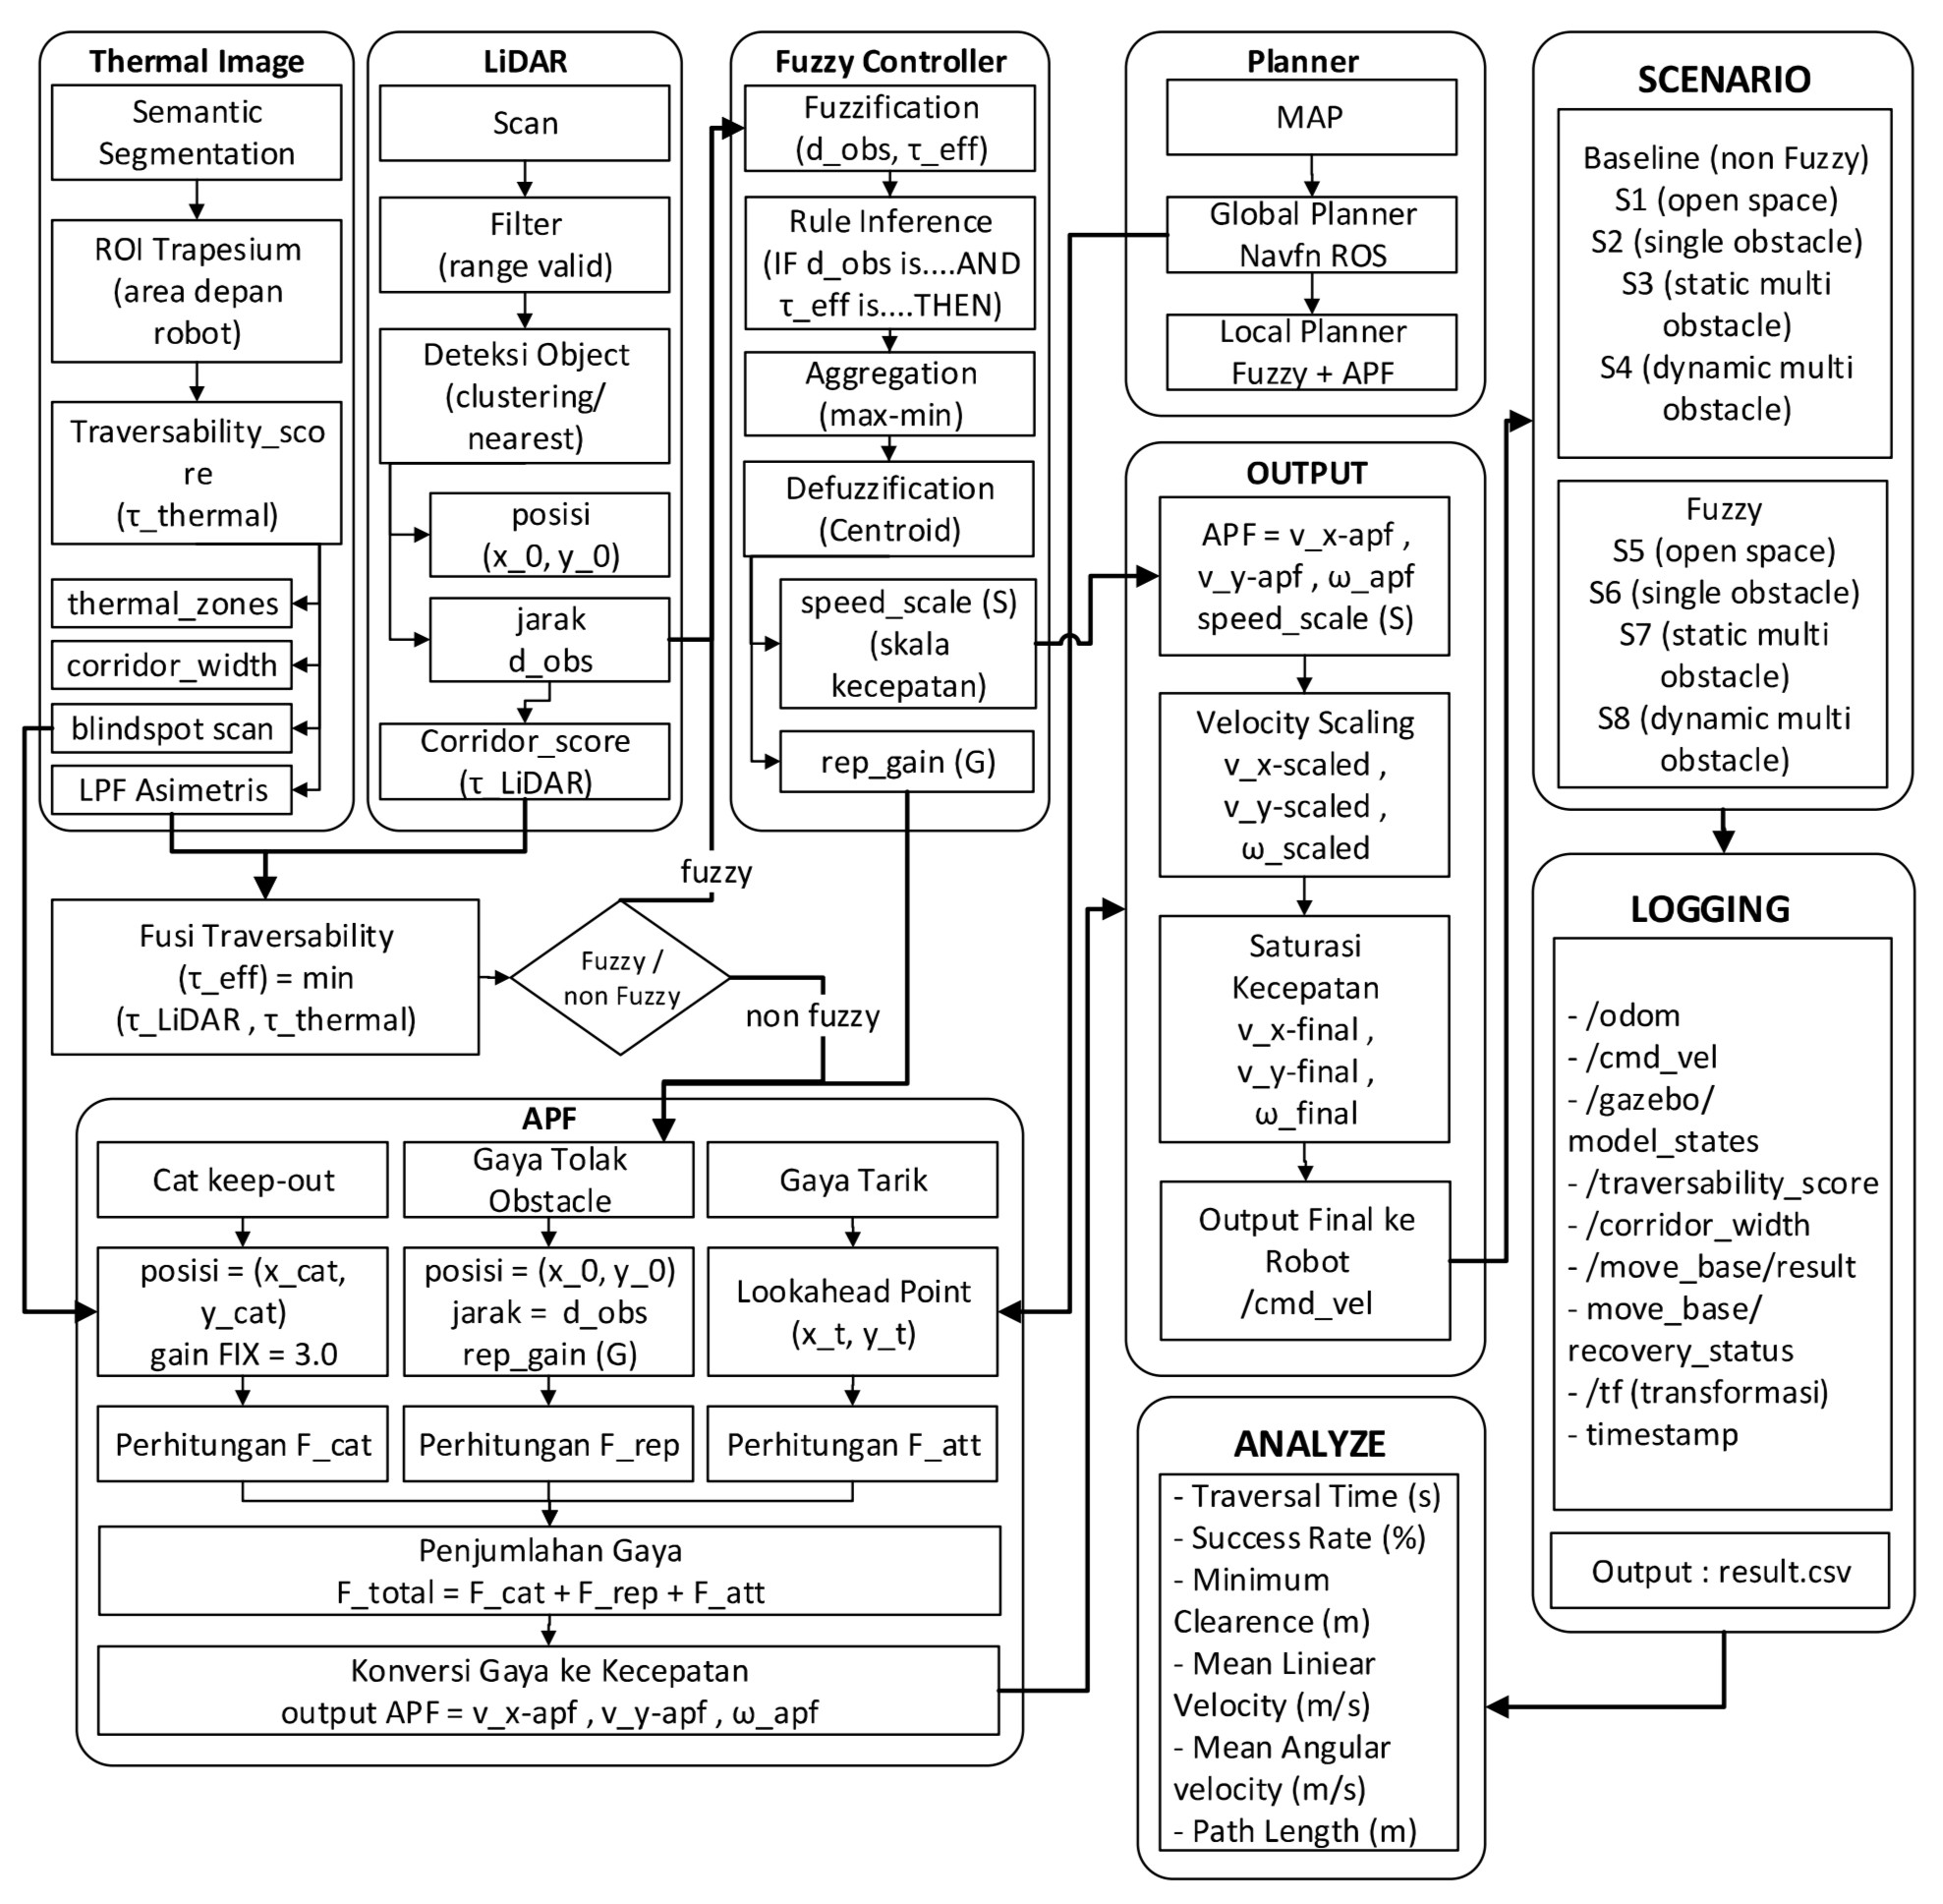
\includegraphics[width=0.7\textwidth]{gambar/3.3_arsitektur_pipeline.jpg}
    \caption{Arsitektur sistem navigasi yang diusulkan.}
    \label{fig:arsitektur_pipeline}
\end{figure}

\subsection{Jalur Pemrosesan Kamera Termal}

Kamera termal menghasilkan citra inframerah berformat grayscale melalui topik \texttt{/the\-rmal/thermal\_camera/image\_raw}. Jalur pemrosesan termal terdiri atas tiga node utama, yaitu \texttt{semantic\_thermal.py}, \texttt{thermal\_feature\_extractor.py}, dan \texttt{thermal\_blindsp\-ot\_to\_scan.py}.

Node \texttt{semantic\_thermal.py} bertugas melakukan segmentasi semantik terhadap citra termal mentah untuk membedakan area obstacle dan area yang dapat dilalui. Hasil segmentasi kemudian diteruskan ke node \texttt{thermal\_feature\_extractor.py} untuk mengekstraksi informasi lingkungan berupa skor traversability termal, lebar koridor, serta kondisi zona navigasi pada area kiri, tengah, dan kanan.

Selain menghasilkan fitur traversability, hasil segmentasi juga digunakan oleh \texttt{thermal\-\_blindspot\_to\_scan.py} untuk membentuk virtual scan yang merepresentasikan obstacle termal pada area blind-spot LiDAR. Pendekatan ini memungkinkan obstacle yang tidak terdeteksi oleh sensor laser tetap dapat dipertimbangkan oleh sistem navigasi tanpa memerlukan perubahan struktur pada ROS Navigation Stack.

\subsection{Jalur Pemrosesan LiDAR}

Sensor LiDAR berfungsi sebagai sumber utama informasi geometris lingkungan. Data hasil pemindaian diterima melalui topik \texttt{/scan} dan digunakan untuk mendeteksi obstacle di sekitar robot serta menghitung karakteristik ruang bebas yang tersedia.

Selain digunakan untuk membangun representasi obstacle pada costmap, data LiDAR juga dimanfaatkan untuk menentukan jarak obstacle terdekat terhadap robot. Informasi tersebut menjadi salah satu variabel penting yang digunakan pada proses pengambilan keputusan navigasi.

Pada penelitian ini, data LiDAR juga digunakan untuk menghitung skor traversability berbasis geometri lingkungan. Nilai traversability tersebut menggambarkan tingkat kemudahan robot untuk bergerak berdasarkan ruang bebas yang tersedia di depan robot. Konsep traversability dipilih karena mampu merangkum kondisi lingkungan ke dalam satu indikator kuantitatif yang lebih mudah digunakan pada proses pengambilan keputusan (\cite{Sevastopoulos2022}).

\subsection{Fusi Traversability dan Pengendali Fuzzy}

Nilai traversability yang dihasilkan oleh kamera termal dan LiDAR tidak digunakan secara terpisah, melainkan digabungkan melalui mekanisme fusi traversability untuk menghasilkan nilai traversability efektif (\textit{effective traversability}). Pendekatan ini memungkinkan sistem mempertimbangkan informasi dari kedua sensor secara bersamaan sebelum mengambil keputusan navigasi.

Nilai traversability efektif selanjutnya digunakan bersama informasi jarak obstacle terdekat sebagai masukan bagi pengendali fuzzy Mamdani (\cite{Mamdani1974}). Melalui proses fuzzifikasi, evaluasi aturan, agregasi, dan defuzzifikasi, sistem menghasilkan dua parameter adaptif yang digunakan pada local planner, yaitu \textit{speed scale} dan \textit{repulsive gain}.

Parameter \textit{speed scale} digunakan untuk menyesuaikan kecepatan linear robot sesuai kondisi lingkungan yang diamati sensor. Sementara itu, parameter \textit{repulsive gain} digunakan untuk mengatur kekuatan gaya tolak obstacle pada APF. Dengan pendekatan ini, perilaku navigasi dapat beradaptasi terhadap perubahan kondisi lingkungan secara lebih fleksibel dibandingkan penggunaan parameter yang bersifat tetap (\cite{Haider2022,Benaicha2026}).

\subsection{Integrasi APF dengan ROS Navigation Stack}

Sistem navigasi yang diusulkan dibangun di atas ROS Navigation Stack yang terdiri atas \textit{map\_server}, \textit{costmap}, \textit{move\_base}, dan \textit{NavfnROS}. Komponen \textit{map\_server} menyediakan peta lingkungan dalam bentuk occupancy grid map yang digunakan sebagai dasar perencanaan lintasan global.

Perencanaan lintasan global dilakukan oleh NavfnROS menggunakan algoritma Dijkstra untuk menghasilkan jalur bebas obstacle dari posisi robot menuju titik tujuan. Jalur global tersebut selanjutnya digunakan oleh APFPlanner sebagai referensi navigasi lokal.

APFPlanner menghitung gaya tarik menuju tujuan dan gaya tolak terhadap obstacle berd\-asarkan informasi yang diperoleh dari sensor. Sebelum dikonversi menjadi perintah kecepatan robot, parameter gaya tolak dan kecepatan linear terlebih dahulu disesuaikan menggunakan keluaran pengendali fuzzy. Hasil akhir proses ini dipublikasikan melalui topik \texttt{/cmd\_vel} dan digunakan untuk menggerakkan robot pada lingkungan simulasi.

\subsection{Konfigurasi Baseline dan Fuzzy}

Untuk mengevaluasi pengaruh pengendali fuzzy terhadap performa navigasi, penelitian ini menggunakan dua konfigurasi sistem yang diuji pada kondisi lingkungan yang identik. Konfigurasi pertama adalah sistem baseline, sedangkan konfigurasi kedua adalah sistem yang dilengkapi mekanisme adaptasi berbasis logika fuzzy.

\begin{table}[H]
\centering
\caption{Kelompok skenario pengujian}
\label{tab:kelompok_skenario}
\begin{tabular}{ll}
\toprule
Kelompok & Skenario \\
\midrule
Baseline & S1, S2, S3, S4 \\
Fuzzy & S5, S6, S7, S8 \\
\bottomrule
\end{tabular}
\end{table}

Pada kedua konfigurasi, sensor LiDAR dan kamera termal tetap diaktifkan sehingga informasi lingkungan yang digunakan sistem bersifat identik. Perbedaan utama terletak pada mekanisme pengendalian yang diterapkan pada APFPlanner.

Konfigurasi baseline menggunakan parameter navigasi yang bersifat tetap, sedangkan konfigurasi fuzzy menggunakan inferensi Mamdani untuk menyesuaikan skala kecepatan dan penguatan gaya tolak berdasarkan kombinasi jarak obstacle dan traversability hasil fusi sensor. Dengan konfigurasi tersebut, pengaruh logika fuzzy terhadap performa navigasi dapat dievaluasi secara langsung tanpa dipengaruhi oleh perubahan konfigurasi sensor maupun lingkungan pengujian.

